% !TEX program = pdflatex
% Order-Book Information & Price Prediction on CFFEX Index Futures
% Detailed research report. Figures are referenced by filename in xn/prediction/;
% add each with \includegraphics where indicated (search "ADD FIG").
\documentclass[11pt]{article}
\usepackage[margin=1in]{geometry}
\usepackage{amsmath,amssymb}
\usepackage{graphicx}
\usepackage{float}
\usepackage{booktabs}
\usepackage{enumitem}
\usepackage{hyperref}
\usepackage{xcolor}
\title{\textbf{Order-Book Information and Price Prediction on CFFEX Index Futures}\\
\large A systematic study of limit-order-book signals (IC, IF, IH, IM)}
\author{}
\date{}

\begin{document}
\maketitle

\begin{abstract}
We test, on four CFFEX stock-index futures (IC 中证500, IF 沪深300, IH 上证50,
IM 中证1000) at 500\,ms Level-1 snapshots over 2020--2026 ($\sim$130M rows), whether the
limit-order book predicts price. We reproduce five classical methods---order-flow imbalance,
queue imbalance, a multi-factor order-flow model, the micro-price, and cross-impact---each with
a strict out-of-sample (OOS) protocol, and follow every signal to a net-of-cost backtest.
The recurring result: order-book signals are \emph{real, OOS-stable, and structural}, but they
live at the \emph{seconds} horizon with \emph{sub-spread} amplitude, so they are not a
taker alpha; their economic value is on the \emph{maker} side (quoting, adverse-selection control)
and, at longer horizons, in \emph{volatility} rather than direction.
\end{abstract}

\section{Data and common method}
\begin{itemize}[leftmargin=*]
  \item \textbf{Table.} DolphinDB \texttt{dfs://hft\_future\_ts}, contracts IC/IF/IH/IM
        (continuous), Level-1: best bid/ask price and size, aggressor volumes, turnover.
  \item \textbf{Notation.} $P_b,P_a$ best bid/ask price; $q_b,q_a$ best bid/ask \emph{size}
        (queue length, in lots); mid $M=(P_b+P_a)/2$; spread $s=P_a-P_b$; tick $\delta=0.2$ pts.
        All prices/quantities are expressed in ticks.
  \item \textbf{Cleaning.} Deduplicate timestamps; drop crossed/locked quotes; sessions
        09:30--11:30 and 13:00--15:00, never differencing across a session boundary; bad-tick
        guard $|\Delta M|>50$ ticks.
  \item \textbf{Estimation.} Pooled OLS via accumulated moments ($X^\top X$, $X^\top y$), so
        full-sample results are exact without holding history in memory.
  \item \textbf{Discipline.} Train 2020-01\,--\,2024-12, \emph{freeze} coefficients, test
        2025-01\,--\,2026-05 (OOS). $R^2$ is the coefficient of determination (fraction of
        variance explained); for high-frequency returns a few percent is a strong, significant signal.
\end{itemize}

\section{Order-book factors}
\begin{enumerate}[leftmargin=*]

  \item \textbf{Volume Order Imbalance (VOI)}\\
  Collect data between consecutive snapshots (consecutive ticks)
  \[
  \Delta V_{\text{bid}} =
  \begin{cases}
  0 & \text{if } P_b \text{ went DOWN (queue died / retreated — ignore)} \\
  q_b - q_{b,\text{prev}} & \text{if } P_b \text{ unchanged (net adds minus cancels/fills)} \\
  q_b & \text{if } P_b \text{ went UP (fresh queue at a better price)}
  \end{cases}
  \]
  \[
  \Delta V_{\text{ask}} = \text{mirror (up}\leftrightarrow\text{down)},\qquad
  \text{VOI} = \Delta V_{\text{bid}} - \Delta V_{\text{ask}}.
  \]
  VOI is the net buying ``effort'' at the top of the book; VOI $>0$ = bid side strengthening.

  \item \textbf{Order Imbalance Ratio (OIR)}
  \[
  \text{OIR} = \frac{q_b-q_a}{q_b+q_a}
  \]
  Three event types that change the book at the top:
  \begin{enumerate}
    \item Limit order: someone posts a new resting order (adds volume)
    \item Cancellation: someone withdraws a resting order (removes volume)
    \item Market order: someone crosses the spread to trade immediately (removes size from the opposite side)
  \end{enumerate}
  As $\text{OIR}\to 1$, $(q_b-q_a)\to(q_b+q_a)$, meaning $q_a$ is significantly smaller than
  $q_b$: the thin ask queue is exhausted first, so the next mid move is up. VOI is the
  \emph{derivative} (flow); OIR is the \emph{level} (stock).

  \item \textbf{Mid-Price Basis (MPB)} --- the only trade-side factor
  \[
  \text{TP}_t = \frac{\Delta \text{Turnover}}{\Delta \text{Volume}\times \text{multiplier}}
  \quad(\text{VWAP of trades this }500\text{ms}),\qquad
  \text{MPB}_t = \text{TP}_t - \tfrac{M_t + M_{t-1}}{2}.
  \]
  Limit orders are free and can be spoofed; \emph{trades cannot lie}. MPB $>0$ (trades printing
  near the ask) $=$ aggressive buying $\Rightarrow$ price rises. Multiplier $=300$ (IF/IH), $200$ (IC/IM).
\end{enumerate}

\section{Direction: queue imbalance (Gould--Bonart 2016)}
For each snapshot we record OIR and the sign of the \emph{next} mid move, and fit a grouped
logistic $P(\text{up}\mid \text{OIR}) = \sigma(a+b\cdot\text{OIR})$.
\\ \textbf{Window:} input = current snapshot; predict the next mid change.
% ADD FIG: fig71_QI概率曲线.png
\begin{figure}[H]\centering
  % 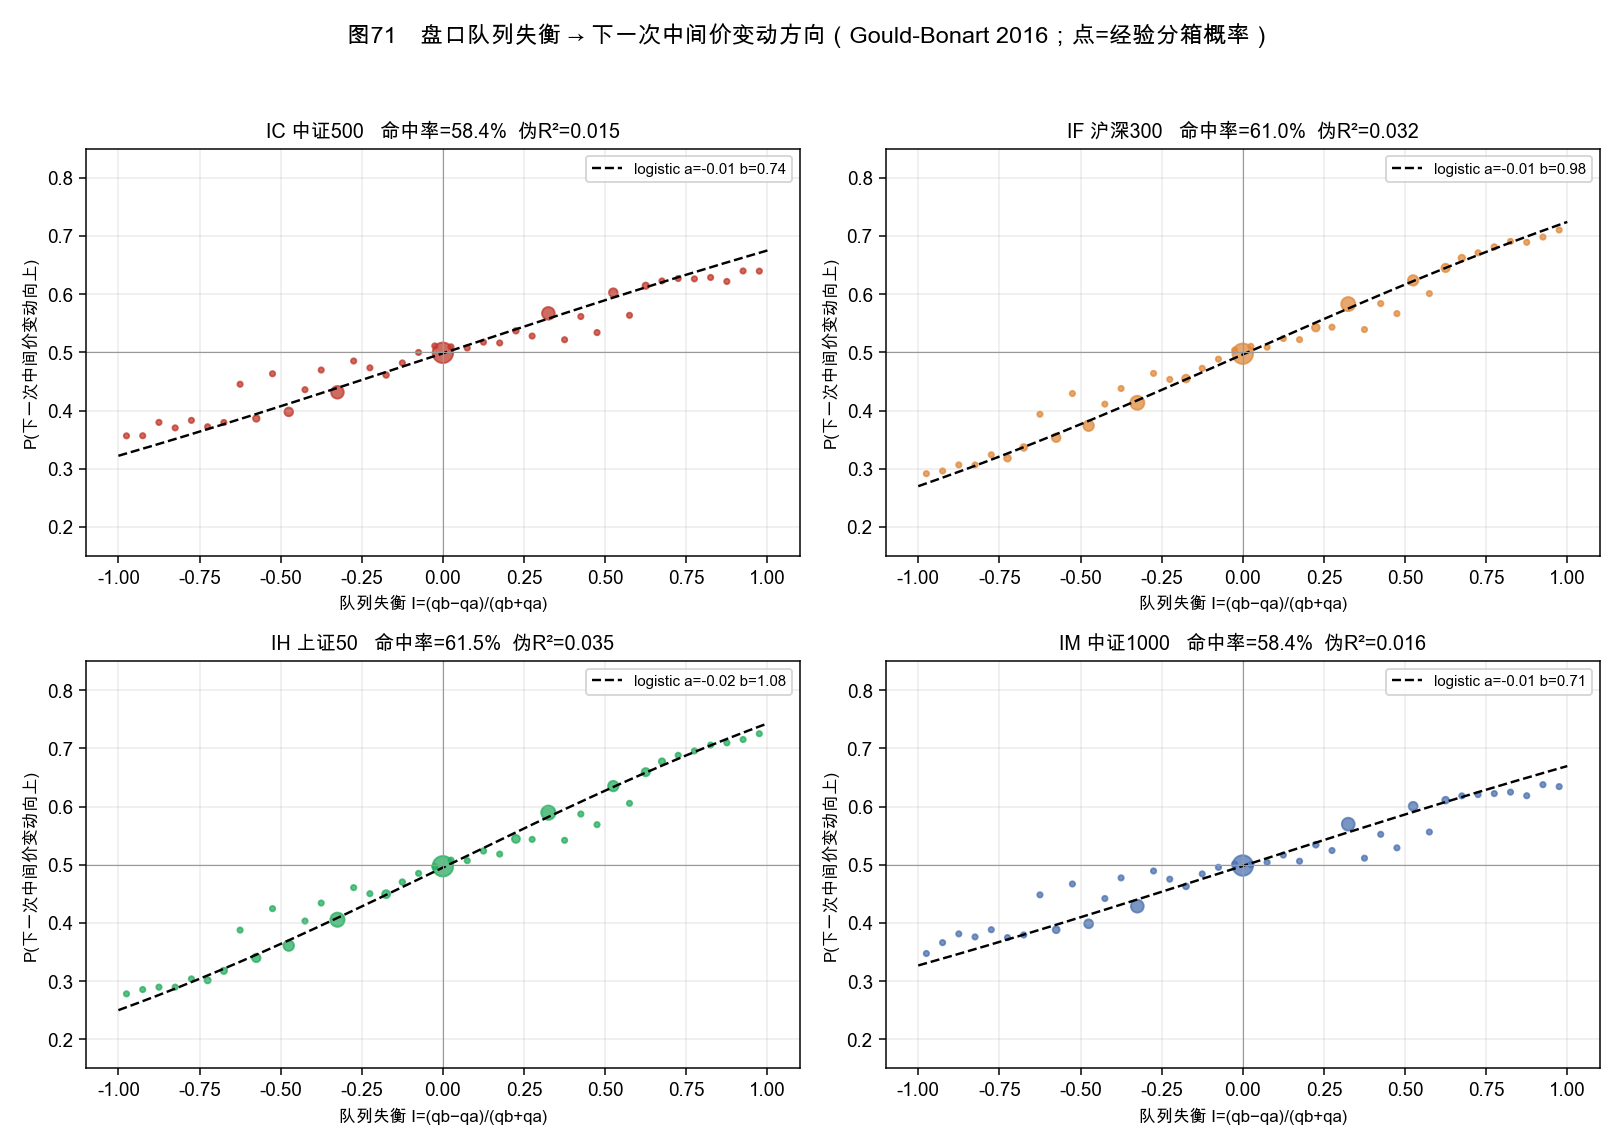
\includegraphics[width=0.7\linewidth]{fig71_QI概率曲线.png}
  \caption{$P(\text{next mid move up})$ vs queue imbalance OIR, per contract, with logistic fit.}
  \label{fig:qi}
\end{figure}
\textbf{Finding:} the curve is monotone for all four contracts; the sign rule
(predict up iff OIR$>0$) hits IH 61.5\%, IF 61.0\%, IC 58.4\%, IM 58.4\%, every month above
50\% for 6.4 years. It is strongest when $s=1$ tick (62.5--66.7\%): the narrower the spread,
the stronger the signal.

\section{Magnitude: multi-factor forecast (Shen 2015)}
Target $y_k(t)=\overline{M}_{t+1..t+k}-M_t$, $k\in\{1,4,20,120\}$ snapshots ($0.5,2,10,60$s).
\begin{align*}
\text{Model A:}\quad & y_k \sim \beta_0 + \textstyle\sum_{l=0}^{5}\beta_l\,\text{VOI}_{t-l}\\
\text{Model B:}\quad & y_k \sim \beta_0 + \textstyle\sum_l \beta_l\tfrac{\text{VOI}_{t-l}}{s_t}
      + \sum_l \gamma_l \tfrac{\text{OIR}_{t-l}}{s_t} + \delta\,\tfrac{\text{MPB}_t}{s_t}
\end{align*}
Six lags ($\approx$3\,s back); dividing by the spread normalizes across spread regimes.
\\ \textbf{Window:} input = last 6 snapshots ($\approx$3\,s); predict the next $k$ snapshots ($0.5$--$60$\,s).
% ADD FIG: fig86_VOI预测散点.png
\begin{figure}[H]\centering
  % 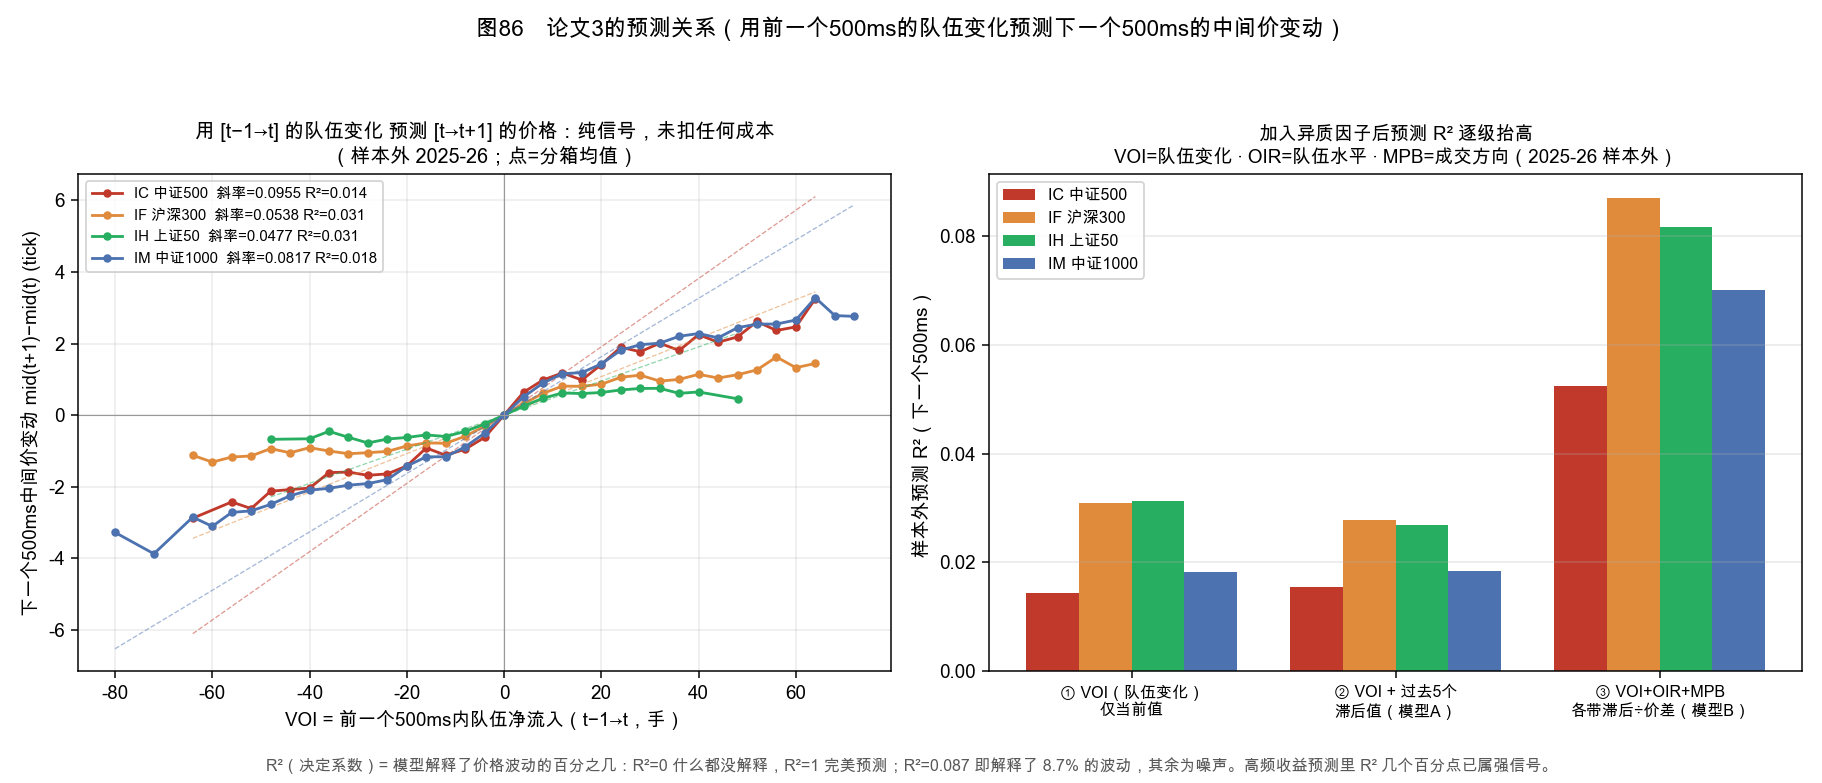
\includegraphics[width=0.9\linewidth]{fig86_VOI预测散点.png}
  \caption{Left: VOI$(t)\to$ next-0.5s mid change (the predictive slope). Right: OOS $R^2$
  ladder --- single VOI $\to$ +lags $\to$ +OIR+MPB.}
  \label{fig:voi}
\end{figure}
\textbf{Finding:} Model B OOS $R^2$ at $k{=}1$: IF 8.7\%, IH 8.2\%, IM 7.0\%, IC 5.2\%; it
decays with horizon (2\,s $\sim$6\%, 10\,s $\sim$1.7\%, 60\,s $\sim$0.3\%) and holds OOS
(frozen $\beta$ $\approx$ refit). MPB alone (windows aligned to VOI) gives OOS $R^2$ 2--4\%
at 0.5\,s, strongest on small-caps, same seconds-decay.
% ADD FIG: fig111_MPB对收益.png  and  fig113_回看窗口.png
The signal is \emph{instantaneous}: varying the look-\emph{back} window (20s--20min) does not
recover it (Fig.~\ref{fig:lookback}); it lives only at instantaneous input $\times$ sub-10s forward.
\begin{figure}[H]\centering
  % 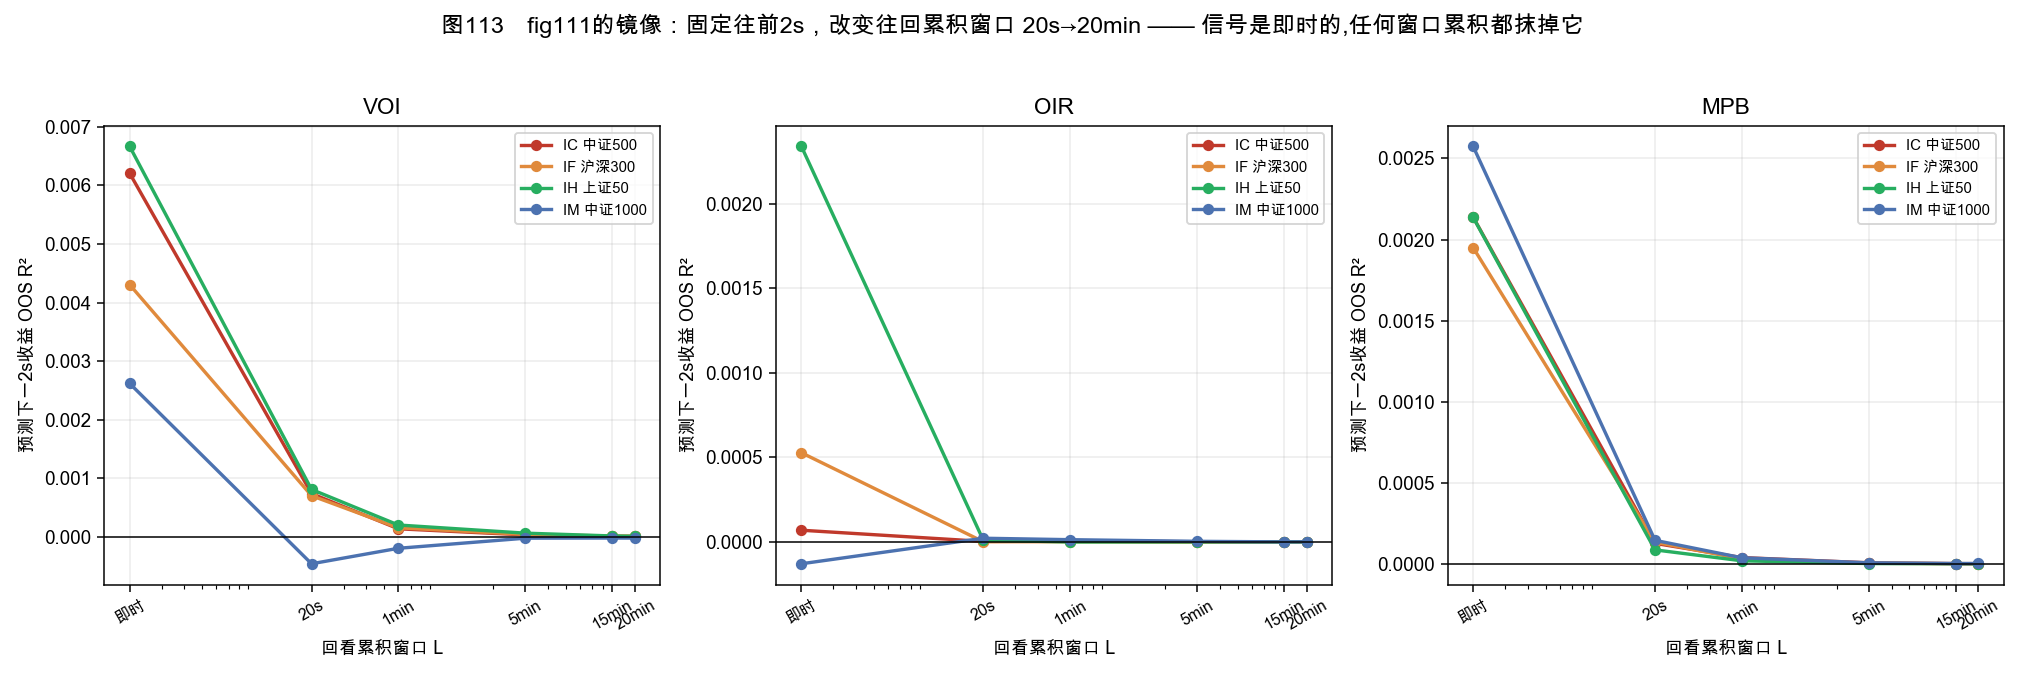
\includegraphics[width=0.9\linewidth]{fig113_回看窗口.png}
  \caption{Mirror test: fix forward $=$ next 2s, vary the accumulation look-back 20s--20min.
  Predictive power collapses the moment you accumulate over any window.}
  \label{fig:lookback}
\end{figure}

\section{Fair value: the micro-price (Stoikov 2018)}
The mid is biased (Sec.~3 shows it drifts predictably). Define the fair price
$P_{\text{micro}} = M + g^*(\text{imbalance},\text{spread})$, with $g^*$ estimated as a
30-state Markov chain (10 imbalance bins $\times$ 3 spread states) so that $P_{\text{micro}}$
is drift-free (a martingale).
% ADD FIG: fig92_条件漂移.png
\begin{figure}[H]\centering
  % 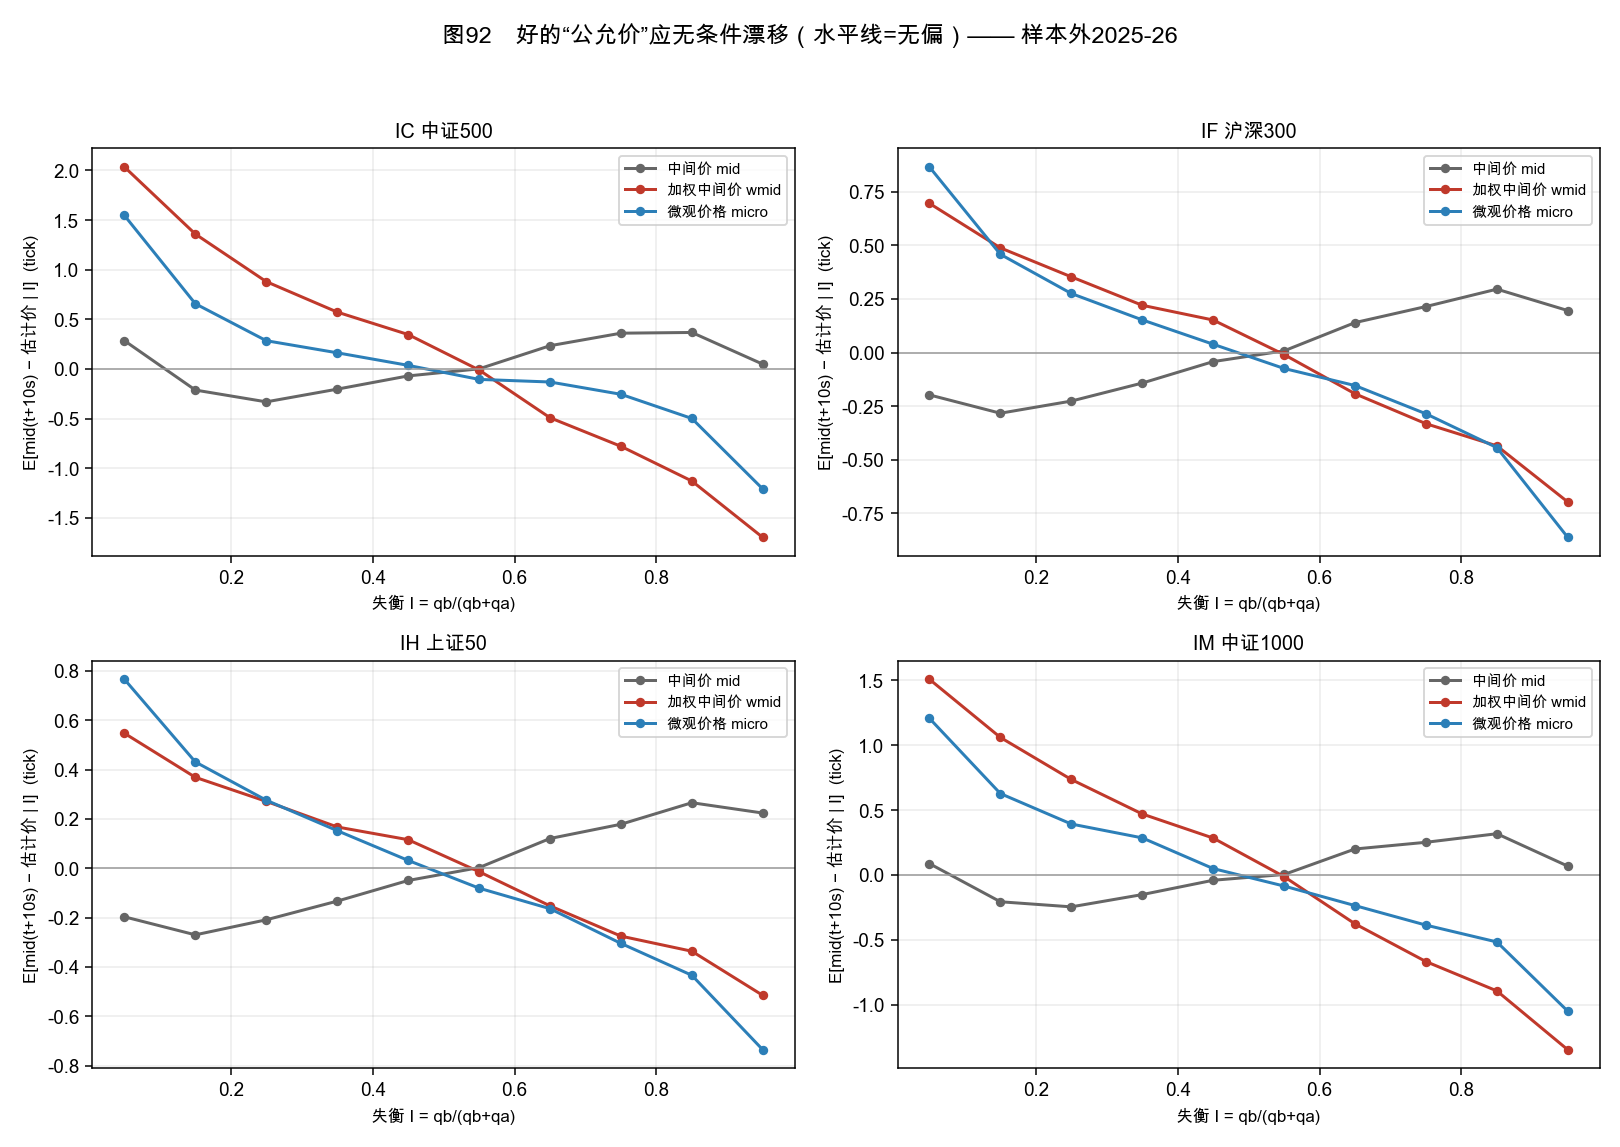
\includegraphics[width=0.8\linewidth]{fig92_条件漂移.png}
  \caption{Conditional future drift $E[M_{t+10s}-P\mid \text{imbalance}]$: mid slopes up
  (under-reacts), weighted-mid slopes down (over-reacts), micro-price is flattest (fairest).}
  \label{fig:micro}
\end{figure}
\textbf{Finding:} shape is structural, but the frozen 5-yr $g^*$ over-corrects out of sample;
a micro-price must be re-estimated on a rolling window.

\section{Cross-contract prediction (Cont--Cucuringu--Zhang 2023)}
Synchronize the four contracts to a common $W$-second grid; ask (i) who leads whom via return
cross-correlation, and (ii) whether $r_i(t{+}1)\sim$ own OFI $+$ others' OFI adds OOS $R^2$.
% ADD FIG: fig101_跨合约领先滞后.png  and  fig103_跨合约OFI系数.png
\begin{figure}[H]\centering
  % 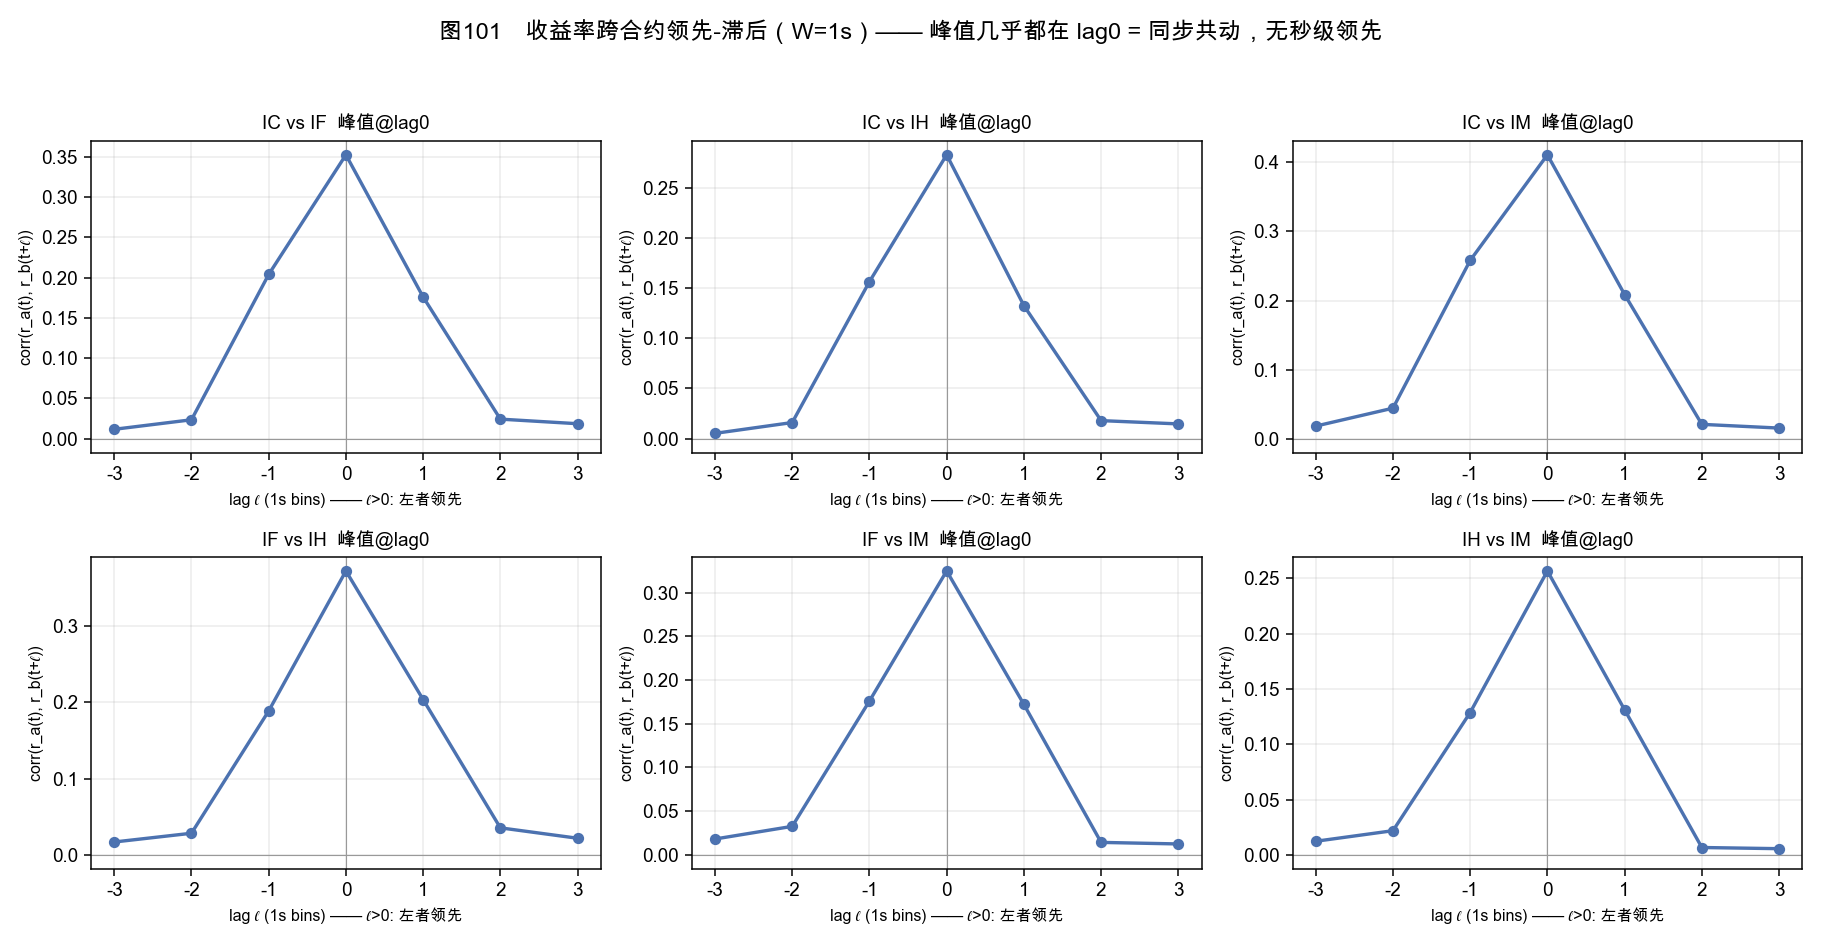
\includegraphics[width=0.9\linewidth]{fig101_跨合约领先滞后.png}
  \caption{Return lead-lag: all six pairs peak at lag 0 --- contemporaneous co-movement, no
  lead-lag above 500\,ms.}
  \label{fig:cross}
\end{figure}
\textbf{Finding:} no lead-lag; cross-OFI $\sim$triples the 1-s OOS $R^2$ (own $\sim$1.7\%
$\to$ +cross 4--6\%), but this is a \emph{common factor} (whole-basket nowcast), not causal.
Zooming to the small-cap pair IC$\leftrightarrow$IM: controlling for IF/IH, $\sim$80\% of the
coupling survives $\Rightarrow$ a genuine small-cap sub-factor (IM faintly leads IC).

\section{From signal to money: backtests}
Every taker backtest uses a five-tier cost ladder (frictionless mid$\to$mid; cross spread;
$+$latency; $+$fees 平昨/平今). Result for the IC$\leftrightarrow$IM signal (1\,s hold):
% ADD FIG: fig105_ICIM回测净利润.png
\begin{figure}[H]\centering
  % 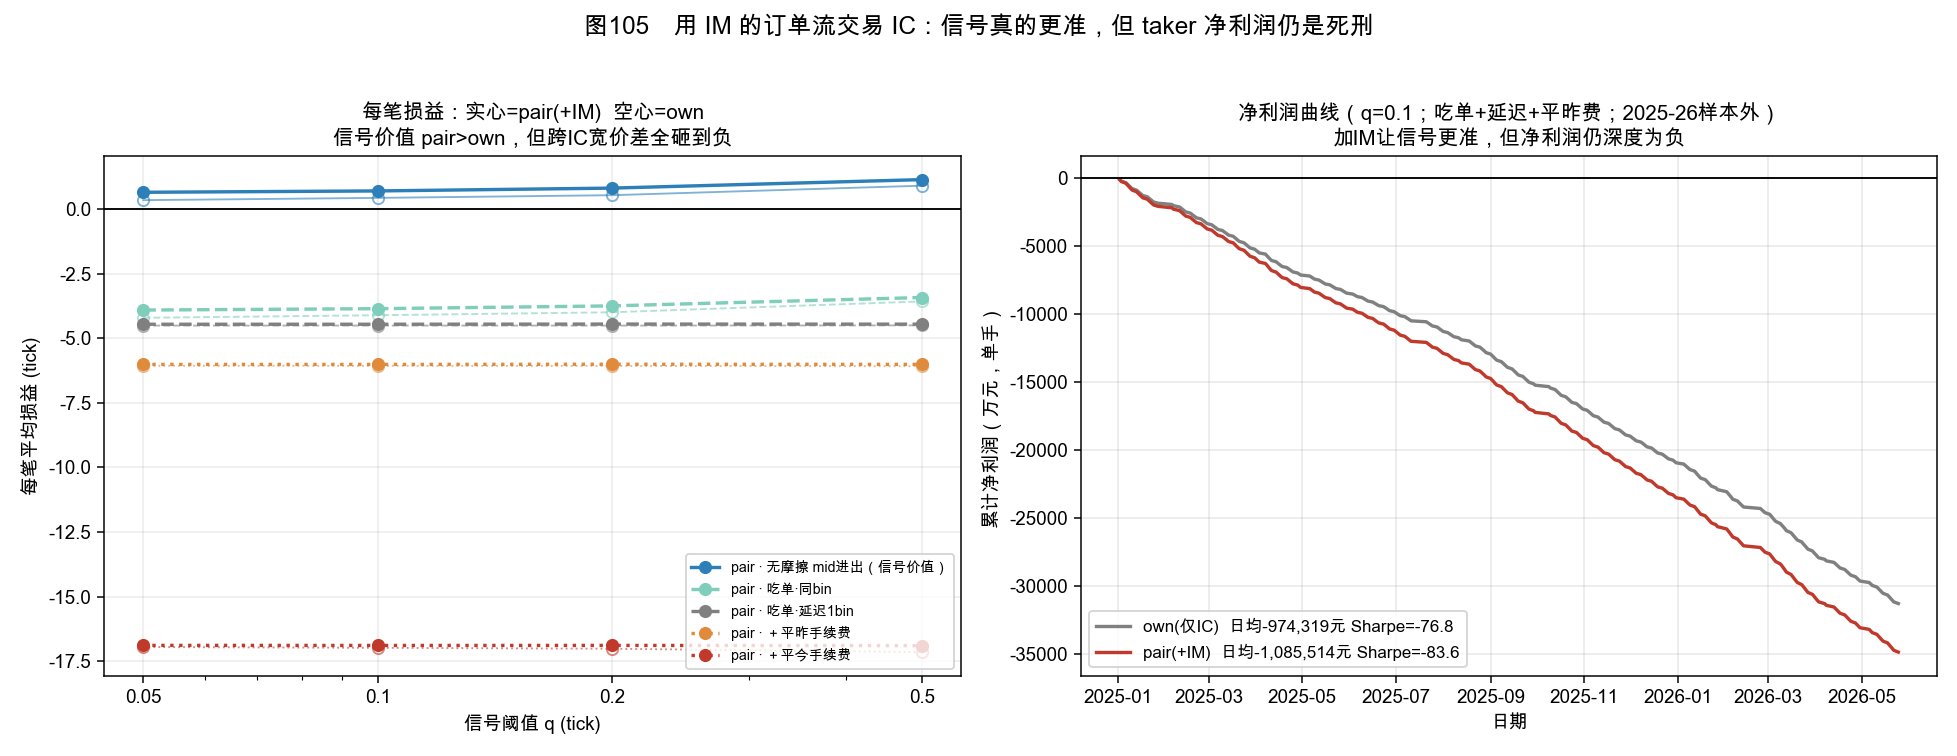
\includegraphics[width=0.9\linewidth]{fig105_ICIM回测净利润.png}
  \caption{Signal value $+0.45\to+0.72$ tick/trade (IM sharpens it), but crossing IC's wide
  spread yields $-6$ to $-17$ tick/trade; the better signal loses \emph{more} (more trades).}
  \label{fig:taker}
\end{figure}
\textbf{Finding (taker):} signal $\ne$ alpha --- a better forecast of a sub-spread move only
lets you lose more confidently.
\\[4pt]
\textbf{Maker capstone.} Rest at $P_b/P_a$; fills inferred from real aggressor volume; P\&L $=$
markout ($M_{t+H}-P_b$ / $P_a-M_{t+H}$). A fair-value $F$ decides which side to quote
($F>M$ $\Rightarrow$ keep bid, pull ask). Compare centers mid / $P_{\text{micro}}$ /
$P_{\text{micro}}+$cross-drift.
% ADD FIG: fig106_做市资本之作.png
\begin{figure}[H]\centering
  % 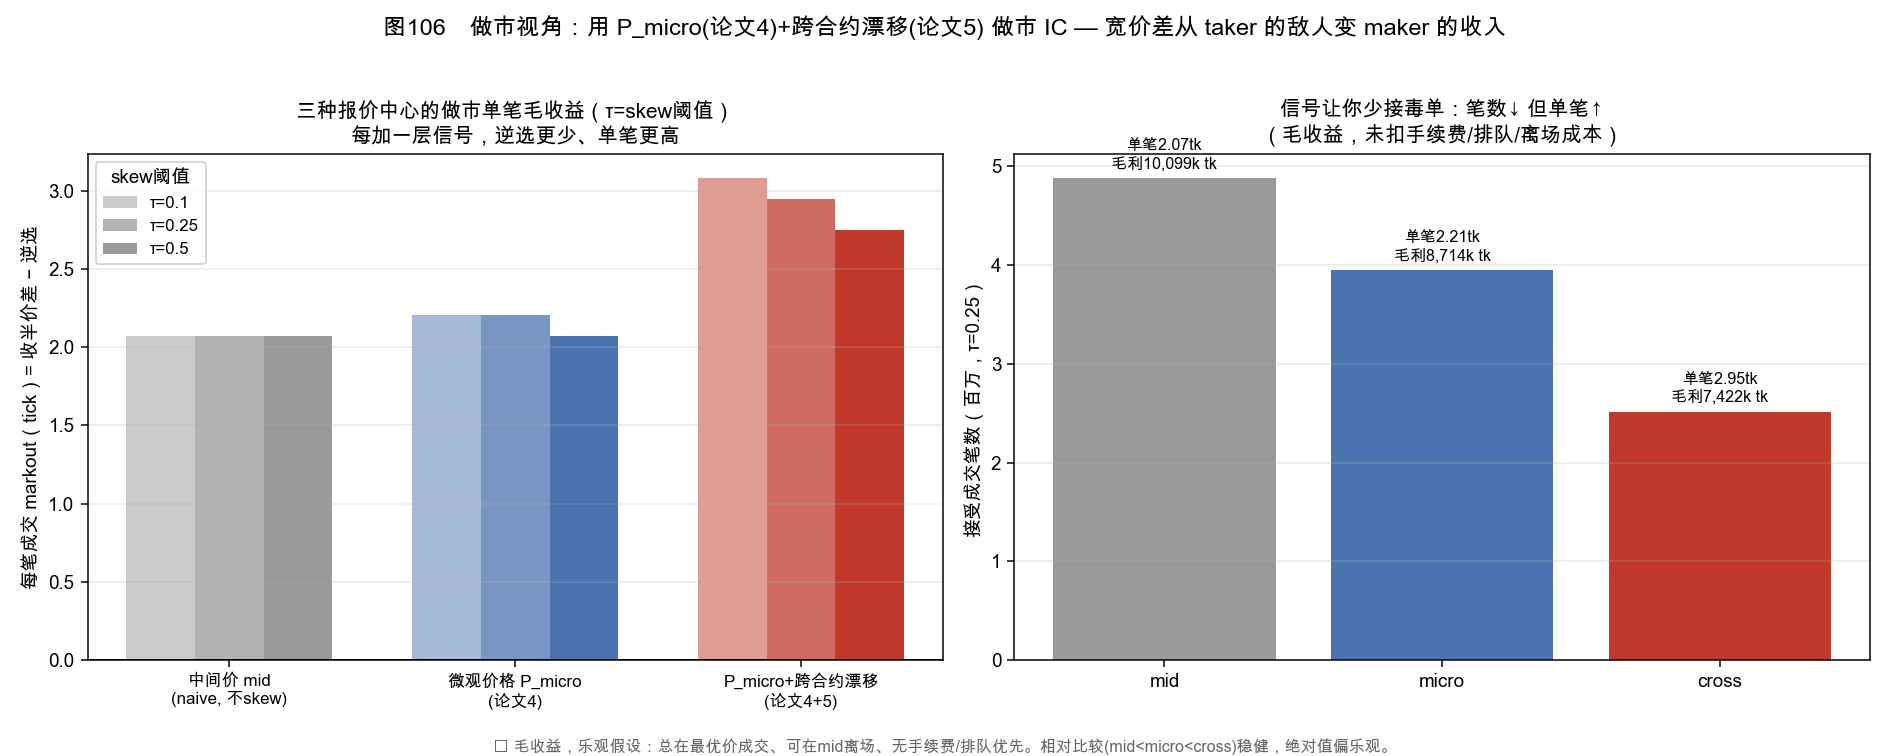
\includegraphics[width=0.9\linewidth]{fig106_做市资本之作.png}
  \caption{Maker markout per fill: mid 2.07 $\to$ micro 2.21 $\to$ cross 2.95 tick (OOS);
  each signal layer pulls toxic fills. Gross, optimistic (no queue priority/fees); the robust
  claim is the relative ordering.}
  \label{fig:maker}
\end{figure}
\textbf{Finding (maker):} the wide spread that costs the taker $-4.5$ tick \emph{pays} the maker
$+2$; $P_{\text{micro}}+$cross-drift cut adverse selection by $\sim$0.9 tick/fill. The money is
in quoting, not predicting.

\section{Extending the horizon: direction vs volatility}
% ADD FIG: fig110_延伸时间轴.png
\begin{figure}[H]\centering
  % 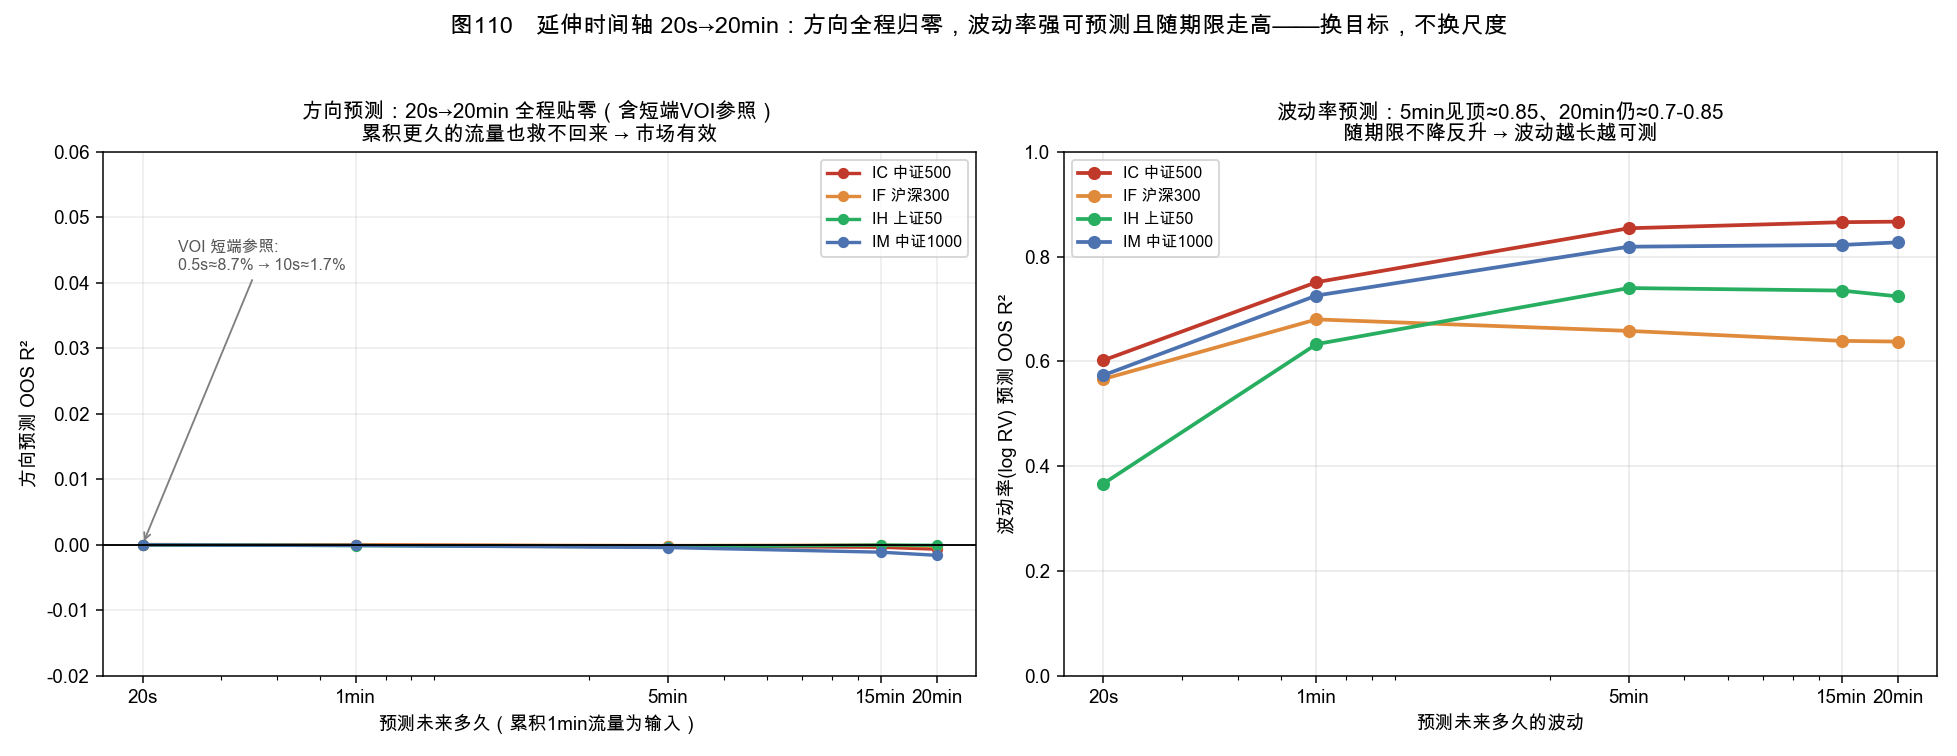
\includegraphics[width=0.95\linewidth]{fig110_延伸时间轴.png}
  \caption{20s--20min. Left: direction OOS $R^2$ is flat on zero everywhere. Right: volatility
  (HAR-RV, log $R\!V$) OOS $R^2$ rises to 0.66--0.87 and stays high; the HAR cascade
  (1/5/30min trailing $R\!V$) beats AR(1).}
  \label{fig:horizon}
\end{figure}
\textbf{Finding:} direction is arbitraged away by minutes; \emph{volatility} is strongly
predictable and \emph{strengthens} with horizon (structure vs noise). Its value is risk:
% ADD FIG: fig112_RV感知做市.png
a RV-aware maker that pulls quotes in predicted-high-vol lowers gross markout (2.93$\to$2.23)
but lowers risk more, raising the risk-adjusted edge $0.40\to0.53$ (Fig.~\ref{fig:volmaker}).
\begin{figure}[H]\centering
  % 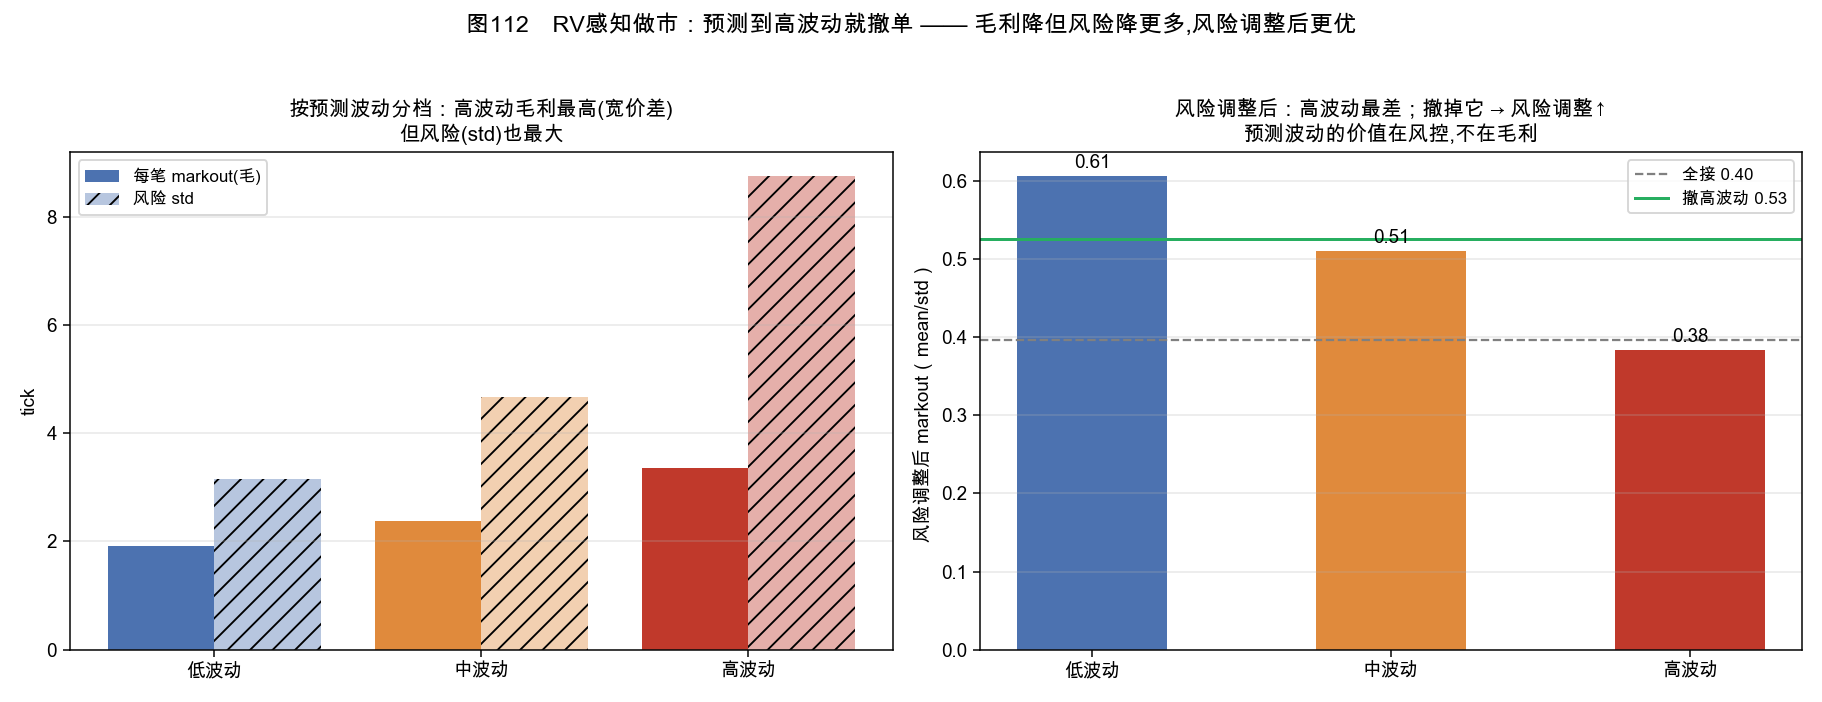
\includegraphics[width=0.9\linewidth]{fig112_RV感知做市.png}
  \caption{Predicting volatility helps the maker through \emph{risk control}, not gross profit.}
  \label{fig:volmaker}
\end{figure}

\section{Conclusion}
The order book carries real, out-of-sample, structurally-stable information, but it lives at the
\emph{seconds} horizon with \emph{sub-spread} amplitude. Hence: (i) no standalone taker alpha;
(ii) genuine value on the \emph{maker} side (micro-price $+$ cross-flow cut adverse selection);
(iii) at longer horizons the predictable object is \emph{volatility}, not direction, and its use
is risk management. Directions with economic content beyond microstructure---basis / basis-momentum,
cross-sectional momentum across the four contracts, and the variance risk premium---are the
natural next factors.

\end{document}
